%  cockshock.tex - documentation source file

%  Written By - Philipp Klaus Krause

%  This program is free software; you can redistribute it and/or modify it
%  under the terms of the GNU General Public License as published by the
%  Free Software Foundation; either version 2, or (at your option) any
%  later version.

%  This program is distributed in the hope that it will be useful,
%  but WITHOUT ANY WARRANTY; without even the implied warranty of
%  MERCHANTABILITY or FITNESS FOR A PARTICULAR PURPOSE.  See the
%  GNU General Public License for more details.

%  You should have received a copy of the GNU General Public License
%  along with this program; if not, write to the Free Software
%  Foundation, 59 Temple Place - Suite 330, Boston, MA 02111-1307, USA.

%  In other words, you are welcome to use, share and improve this program.
%  You are forbidden to forbid anyone else to use, share and improve
%  what you give them.   Help stamp out software-hoarding!

\documentclass[a4paper]{article}
\usepackage{xltxtra}
\usepackage{siunitx}
\usepackage[pdftitle={Cock Shock},pdfauthor={Philipp Klaus Krause}]{hyperref}

\begin{document}
\title{Cock Shock}
\author{Philipp Klaus Krause}

\maketitle

\section{Introduction}

The Cock Shock is a remote-controlled electric cock-and-ball-torture device. There is only a small number of such devices currently commercially available, and the Cock Shock seems to be the most easily available and affordable one.

However, it has various shortcomings, both in documentation and the device itself.

Reverse engineering will result in better documentation, such as this document, and hopefully in hacks to address the device's shortcomings.

\section{What is the Cock Shock?}

The Cock Shock is a remote-controlled electric cock-and-ball-torture device by Master Series. It consists of a remote control and a shock unit. The shock unit is meant to be attached to male genitals and can provide electric shocks and vibration. The remote control sends commands to the shock unit via 434 MHz RF. There is some safety designed into the protocol to avoid accidental activation of the shock unit by other nearby 434 MHz devices. There is no security, so a deliberate activation of the shock unit by an attacker (e.g. a replay attack using a software-defined radio) would be easy.

\section{What is the Problem?}

The Cock Shock is badly documented by the manufacturer, and has some shortcomings in functionality.

As can be seen from reviews (e.g. on www.amazon.com and on some blogs), some users didn't get instructions or maybe didn't notice the small folded piece of paper that contains the instructions, resulting in them being unable to get the device to work. Other users have trouble due to undocumented functionality, such as the 3-minute auto-shutdown timeout.

Many also miss some functionality, such as setting the shock level:

\begin{quotation}
I would have liked there to be two, or three, different levels of intensity for the jolts. Just to perhaps tease, or train, my slaves up through several levels of shock, rather than have them cry their safe word so quickly. So, consequently, all of my “cock-shocker” sessions have been quite short so far! […] But, I haven’t yet had any of the subs I’ve used it on, be able to take more than two or three jolts before they’ve cried their “safe word”\cite{Ellison2016}
\end{quotation}

\begin{quotation}
I’ve used a fair few electro sex toys and can use cock loops at maximum output on the powerboxes I have – this feels nothing like them at all. Where they can feel like a nice powerful vibration this feels more like how I imagine a taser feels, it is a powerful jolt that even my masochistic slave was fearful of – it hurts that much.\cite{Decerous2016}
\end{quotation}

Being able to disable the 3-minute auto-shutdown timeout would also be useful.

\section{Using the Cock Shock}

The manufacturer's instructions are rather short and incomplete:

\begin{quotation}
Instructions:

To use the Cock Shock, first insert a 9v battery (included) into the remote control. Second, unscrew the electro contact points on the shock unit and remove the inner plate to reveal the battery compartment. Insert two AAA batteries (not included).

A red and green light should come on in the shock unit, and the red light should be flashing. At this time hit either the shock or vibrate button to pair the remote to the shock unit. Reinstall the inner plate, and screw the electro contact points back on.

Now strap the shock unit to his junk in whatever way you see fit, making sure that the contact points are pressing firmly into his skin. Now he either behaves, or you discipline him.\cite{MasterSeriesCockShockInstructions}
\end{quotation}

\begin{figure}
	\centerline{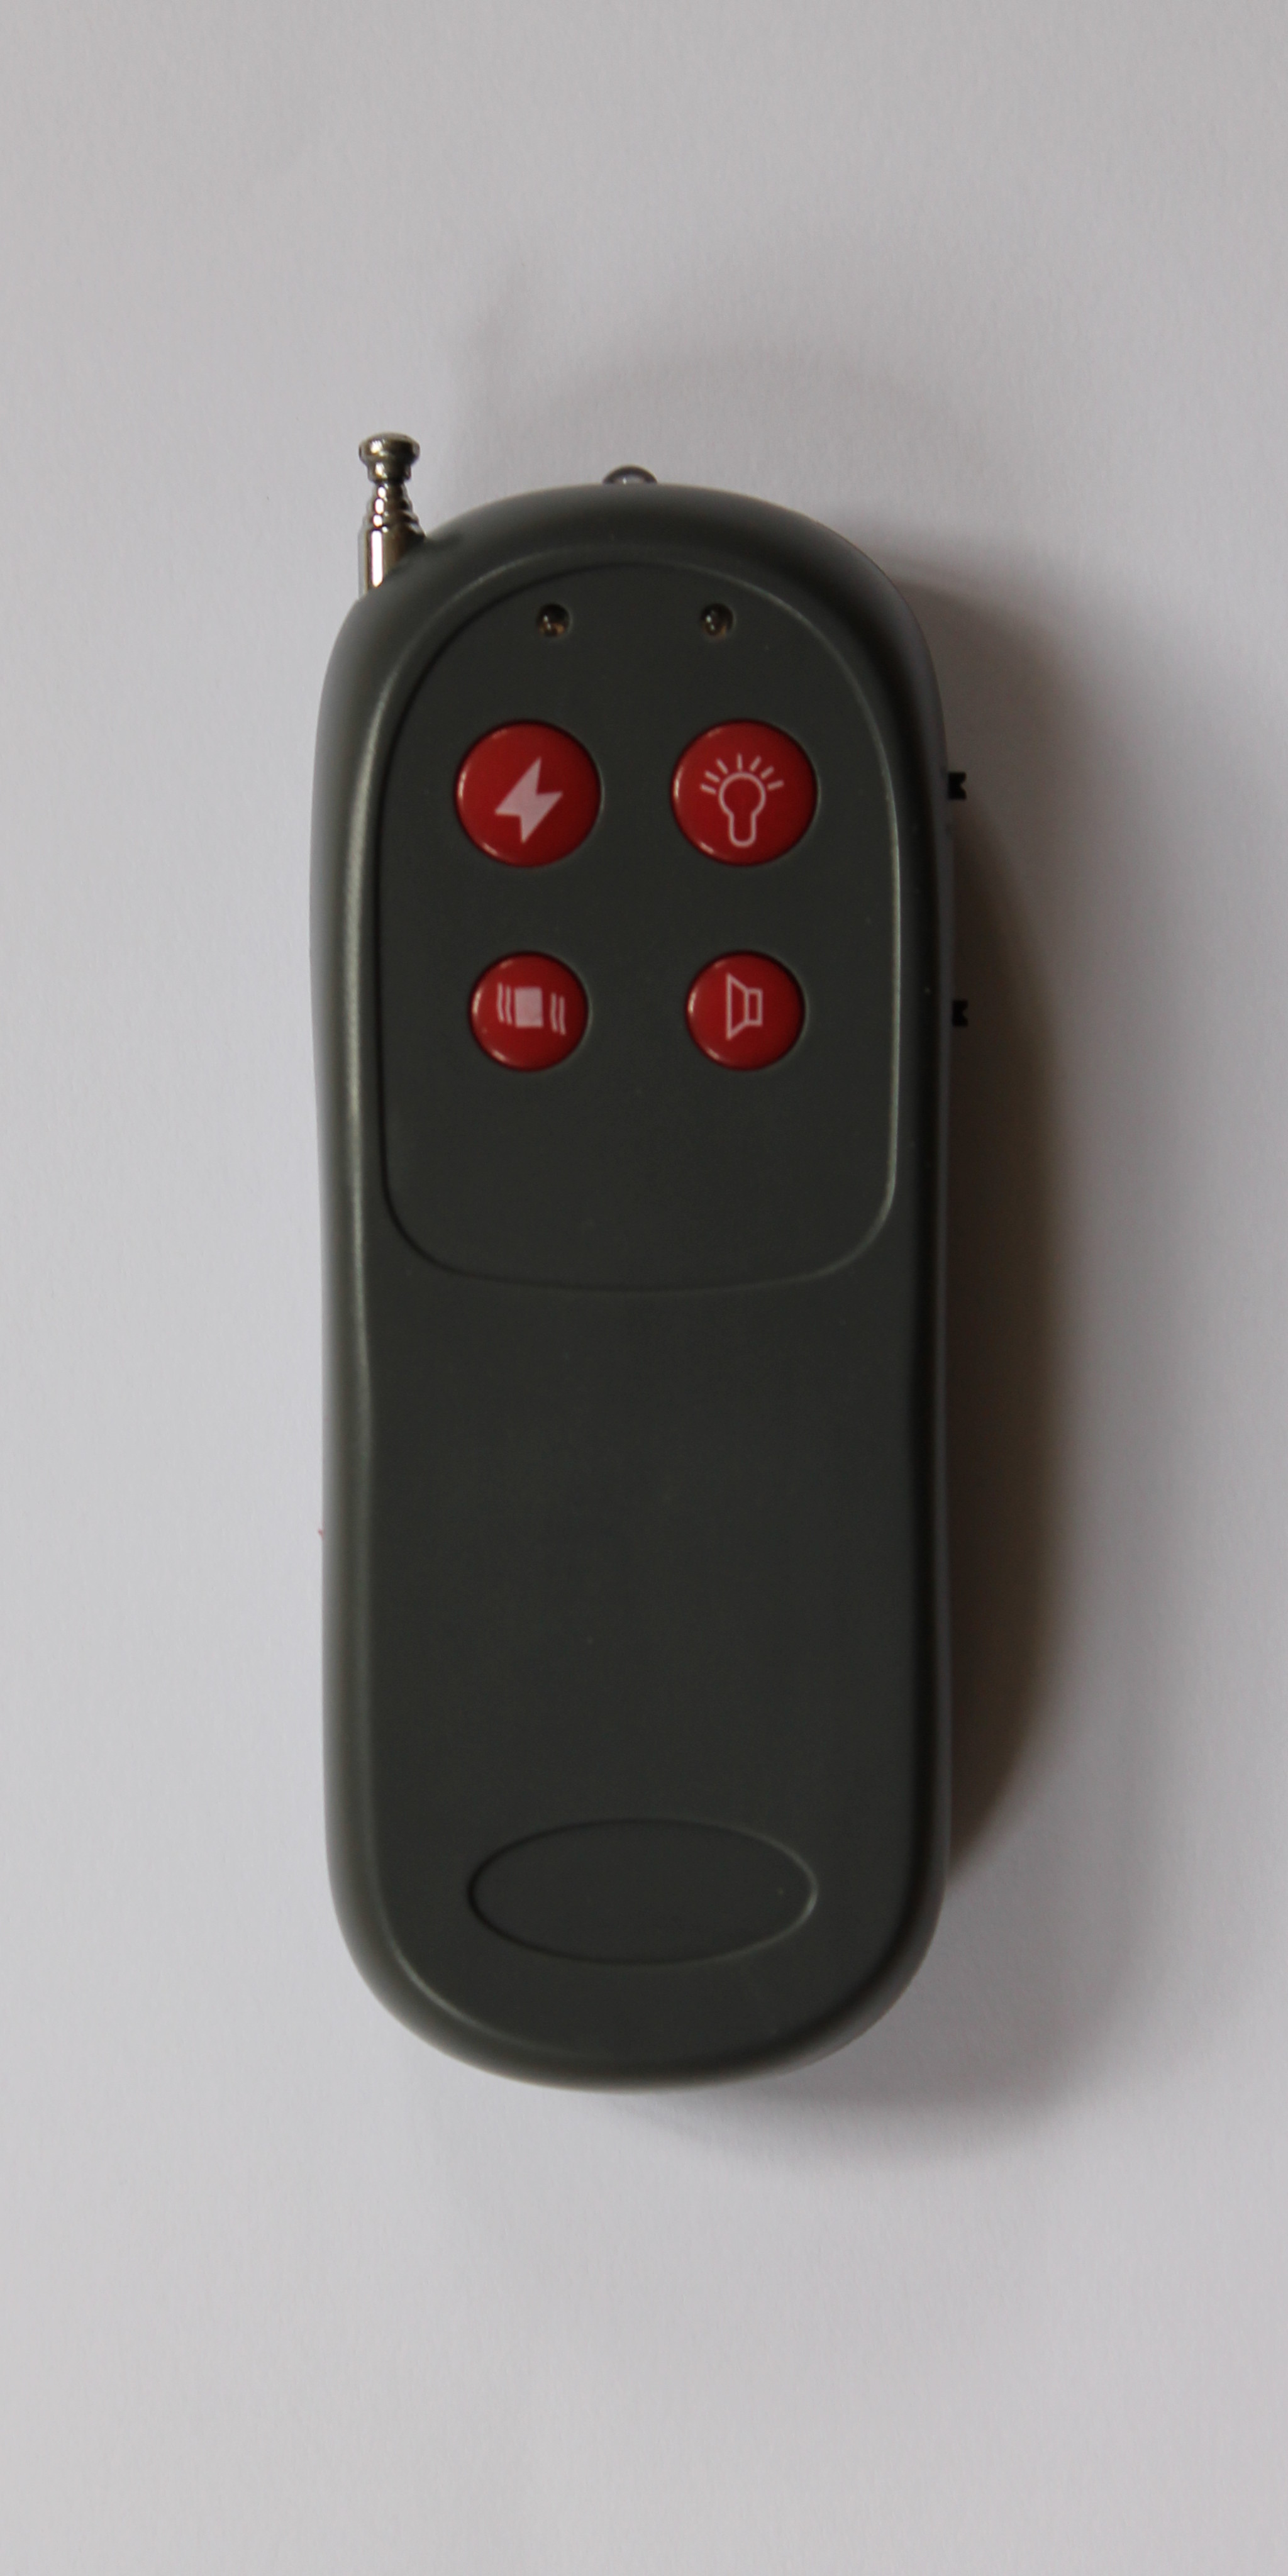
\includegraphics[scale=0.05]{remotecontrol.jpeg}}
	\caption{\label{remotecontrol}Remote Control}
\end{figure}

The remote control (see Figure \ref{remotecontrol}) has 4 buttons (Shock, Light, Vibrate, Sound) and 2 switches (On/Off, Volume). The Shock and Vibrate buttons send commands to the shock unit via RF. The Light button shines a blueish light from the front of the remote control. The Sound button sounds a bird noise from the back of the remote control, the volume depends on the setting of the volume switch. The On/Off button is mostly useful to prevent accidental triggering of any functions. The remote control consumes virtually no power even when switched on as long as no buttons are pressed (see Figure \ref{remotepower}). There also are three LEDs, the top one for the light, the right one to indicate that the sound should be active (at low battery voltage, the sound can be inaudible, but the LED wills till light up), the left one to indicate that a command is being sent to the shock unit. The antenna can be extended to increase range.

\begin{figure*}[h]
	\centerline{\begin{tabular}{|l|r|r|r|r|r|r|r|r|}
	\hline
	Bat.\ volt. & Off & Idle & Shock & Light & Vibrate & Sound- & Sound & Sound+ \\
	\hline
	\hline
	8.4 V & < .1 µA & < .1 µA & 30 mA & 36 mA & 35 mA & 10 mA & 30 mA & 110 mA\\
	\hline
	9.0 V & < .1 µA & < .1 µA & 35 mA & 40 mA & 37 mA & 10 mA & 30 mA & 80 mA\\
	\hline
	\end{tabular}}
	\caption{\label{remotepower}Measured battery current draw of remote control at the nominal voltages of NiMH and Alkaline batteries}
\end{figure*}

The shock unit has two electrodes, for making contact with skin. While they have a good shape for their purpose, using a conductive electrode gel can further reduce resistance between the electrodes and the body. When the shock unit receives no commands for about 3 minutes, it goes into shutdown, reducing power consumption by about 20\% (see Figure~\ref{shockunitpower}). In shutdown mode, the shock unit will not receive any commands from the remote control. The shock unit has a tilt sensor and can be brought out of shutdown mode by moving it. When the unit is not in use, the battery should be taken out, as the high current draw will quickly empty the battery even when in shutdown.

\begin{figure*}[h]
	\centerline{\begin{tabular}{|l|r|r|r|r|}
	\hline
	Bat.\ volt. & Idle & Shutdown & Shock & Vibrate \\
	\hline
	\hline
	2.4 V & 54 mA & 41 mA & 156 mA & 140 mA\\
	\hline
	3.0 V & 52 mA & 41 mA & 170 mA & 160 mA\\
	\hline
	3.3 V & 51 mA & 41 mA & 170 mA & 172 mA \\
	\hline
	\end{tabular}}
	\caption{\label{shockunitpower}Measured battery current draw of shock unit at the nominal voltages of NiMH, Alkaline and NiZn batteries}
\end{figure*}

\section{The Remote Control}

The remote control contains Princeton Technology PT2240B Encoder, which encodes 25-bit code words in a form suitable for RF modulation. Each code word consists of a 20-bit little endian address, followed by a 4-bit big-endian data nibble followed by a sync bit. The highest data bit indicates a shock command, the second-highest indicates a vibrate command, the lower 2 data bits are always 0 (the respective pins on the PT2240B have pull-down resistors).

TODO: PCB pictures.

TODO: Schematics.

\section{The Shock Unit}

The shock unit electronics consist of three parts: A RF module, the main part and the high-voltage module. The RF module consists of a separate PCB interfaced via 3 pins to the main module. The high-voltage part interfaces via two PCB traces to the main module. Both the RF module and the main module contain an IC. On both ICs, the markings have been sanded off. the main module also features a vibrator and a tilt switch.

The RF module is almost identical to the reference circuit in the datasheet of the HOPERF RF83C RF receiver IC. Thus, the IC is most likely a RF83C, though other RF ICs with a compatible pinout, such as the Micrel MICRF002/RF022 cannot be ruled out.

\begin{figure*}[h]
	\centerline{\begin{tabular}{|l|l|}
	\hline
	Pin & Use \\
	\hline
	\hline
	1 & Not connected\\
	\hline
	2 & Not connected\\
	\hline
	3 & Not connected\\
	\hline
	4 & 3.3 V\\
	\hline
	5 & Output to vibrator, connected to transistor via 2.2 k\si{\ohm} resistor\\
	\hline
	6 & Output to vibrator, connected to transistor via 2.2 k\si{\ohm} resistor\\
	\hline
	7 & Data input from RF module\\
	\hline
	8 & Output to high-voltage module, connected to transistor via 150 \si{\ohm} resistor\\
	\hline
	9 & Output to vibrator, connected to transistor via 2.2 k\si{\ohm} resistor\\
	\hline
	10 & Input from tilt sensor\\
	\hline
	11 & GND\\
	\hline
	12 & Output, connected to LED via 1 k\si{\ohm} resistor\\
	\hline
	13 & Input, connected to battery voltage via 0 \si{\ohm} resistor\\
	\hline
	14 & Not connected\\
	\hline
	\end{tabular}}
	\caption{\label{mainmoduleic}Pinout on the unmarked IC on the main module}
\end{figure*}

The main module contains an SOIC-14 IC which is probably a µC. The unusual pinout could help identify it (see Figure~\ref{mainmoduleic}). So far, the EM78P153A has been identified as a possibility.

TODO: PCB pictures.

TODO: Schematics.

TODO: Measure shock voltage and waveform. Under no load, the voltage is in excess of 2000V (upper limit of measurement device used so far).

\section{Hack: Disable the 3-minute auto-shutdown timeout}

A simple modification would be replacing the tilt switch in the shock unit by a slow (0.01 Hz to 10 Hz) Oscillator to disable the 3-minute auto-shutdown timeout.

The oscillator could be built from just three small components: A 74LVC1G14 inverting Schmitt-trigger buffer, a 1 µF capacitor and a 100 \si{\ohm} resistor.

\section{Hack: Adjustable shock intensity}

So far, this is just an idea.

If the pulse output for shocks from the µC can be used to set the shock intensity (e.g. by charging some capacitors just partially), a more advanced modification would be to replace the µC in the shock unit by a different one programmed to use the lower bits of the received data for the shock intensity (and also get rid of the 3-minute auto-shutdown timeout at the same time). This would also require a modification of the remote control, e.g. connecting the volume switch to the encoder inputs for the lower data bits.

\bibliographystyle{plain}
\bibliography{cockshock}

\end{document}

